\chapter{Entwurf}\label{ch:entwurf}
In den folgenden Abschnitten werden die inhaltlichen Anforderungen bezüglich der Projektziele beschrieben. Diese werden in Form von Personas und User Stories dargestellt. Dazu passend werden anschließend die grafischen Anforderungen mithilfe von einem Styleguide und einem Prototypen verdeutlicht. Zuletzt werden unterschiedliche Entwicklungsumgebungen und Frameworks evaluiert, um so zu erschließen, welche sich am besten für das Projekt eignen.

\section{Inhaltliche Anforderungen}\label{inhaltliche_anforderungen}
Um de Aufteilung und Erstellung der inhaltlichen Anforderungen einfacher zu gestalten, wurden zunächst Personas entwickelt. Die Persona-Methode ist im UX-Design eine beliebte Herangehensweise, um für alle Projektbeteiligten eine gewisse Nähe zu den Nutzergruppen herzustellen.

Bei Personas handelt es sich um fiktive Personen, die als Stellvertreter für eine bestimmte Zielgruppe stehen. Sie werden anhand von Informationen über diese Gruppen entwickelt. Da TraWo ursprünglich für Nutzer von allen Altersgruppen gedacht ist und sich somit an mehrere Zielgruppen richtet, soll durch die Personas klar werden welche hierbei besonders im Vordergrund stehen: Eltern und Kinder.

Des Weiteren bietet das Persona-Konzept gegenüber der Arbeit mit gesichtslosen Gruppen an zahlreichen Vorteilen und ist somit eine bessere Entscheidung für unser Team. Eines dieser Vorteile ist wie bereits mehrmals angedeutet die Veranschaulichung der Zielgruppen, wonach sich das Projekt richtet. Dieses Merkmal ist nicht nur einer der wichtigsten Erkennungen, sondern auch gleichzeitig eines der Ziele des Persona-Konzepts. Während des Arbeitsprozesses helfen Personas vor allem dabei, die eigentliche Zielgruppe nicht aus den Augen zu verlieren. Sie bieten nicht nur Vorteile bezüglich der Zielgruppen, sondern fördert auch gleichzeitig den kreativen Prozess im Laufe der Entwicklung. Außerdem werden im Gegensatz zu einer pauschalen Gruppe Bedürfnisse von Personas besser an das Entwicklerteam übermittelt.

Doch wie entwickelt man eigentlich Personas? Es handelt sich um eine Art Steckbrief eines prototypischen Nutzers, welcher relevante Informationen bezüglich des Projekts enthält. Dazu gehören beispielsweise demografische Daten, Vorlieben am Produkt, Schwierigkeiten bei der Nutzung, Motivation zur Nutzung sowie Handlungskontexte bezogen auf das Produkt. In dem Fall von TraWo werden nur die wichtigsten Merkmale die im Verlauf der Entwicklung von Bedeutung sind verwendet.

Wie in Abbildung \ref{fig:persona_thorsten} zu sehen ist, handelt es sich bei der ersten Persona um Thorsten. Er ist acht Jahre alt und besucht aktuell die Grundschule. In seiner Freizeit verbringt er sehr gerne Zeit am Tablet. Aus diesem Grund wünscht er sich eine Anwendung, die ihm das Lernen mit einem Buch durch ein Spiel ersetzt.

Bei der nächsten Persona, die in Abbildung \ref{fig:persona_mark} zu erkennen ist, handelt es sich um Mark. Er ist 38 Jahre alt und ist momentan in der IT-Branche tätig. Er hat einen achtjährigen Sohn namens Thorsten. Aus seiner Liebe zu Computern ist es Mark besonders wichtig, seinen Sohn auch auf eine technische Art und Weise beim Lernen zu unterstützen und somit seine Bildung zu fördern. Er sucht nach einem Produkt, welches nicht nur zur Unterstützung beim Lernen dient, sondern auch die Motivation seines Sohnes erweckt.

Im Anschluss können mithilfe der zuvor entwickelten Personas Anforderungen in Form von User Stories erstellt werden.

Bei einer User Story handelt es sich um eine kurze Erläuterung einer Funktion, die aus der Sicht eines Nutzers oder wie in diesem Fall einer Persona geschrieben wurde. Warum wir uns für User Stories entschieden haben, liegt vor allem daran, dass sie für jeden aus dem Team leicht zu verstehen sind. Dabei ist es zu beachten, die Aufgaben so zu formulieren, dass sie auch von Beteiligten ohne technische Hintergründe verstanden werden können. Außerdem ist es so möglich, die unterschiedlichen Anforderungen in kleinere Aufgaben zu unterteilen, um so bessere Ergebnisse bis zu den regelmäßigen Sprints zu erhalten. Nach der Erstellung der User Stories werden im Team \textquote{Story Points} vergeben. Diese beschreiben die Größe und den damit entstehenden Aufwand einer User Story. Auf diese Funktion wurde in unserem Fall bewusst verzichtet, da keine große Anzahl an Anforderungen vorhanden ist. Stattdessen wurde entschieden, die Aufgaben nach Wichtigkeit zu sortieren. So war es einfacher für das Team herauszufinden, welche Aufgaben in dem Moment Vorrang haben. 

Im Bezug auf TraWo wurde die Persona Mark zur Erstellung eines Szenarios genutzt. Dieses soll dabei helfen, einen Einblick in das vorliegende Problem zu bekommen. Aus diesem Problem wurden anschließend User Stories entwickelt, die aus der Sicht von Thorsten formuliert sind.

\textbf{Szenario:}
Mark möchte eine App für seinen Sohn, die ihm auf eine spielerische Art und Weise grafisches Allgemeinwissen beibringt.

\textbf{User Stories:}
\begin{itemize}
\item \textquote{Als Thorsten möchte ich innerhalb der App Zugriff auf ein Menü haben.}
\item \textquote{Als Thorsten möchte ich ein On-Boarding, dass mir kurz erklärt, wie die App funktioniert.}
\item \textquote{Als Thorsten möchte ich mich zwischen dem Informationsteil und dem Spielteil entscheiden können, damit ich auch ohne Benutzung der Kamera Zugriff auf die Informationen zu den Ländern habe.}
\item \textquote{Als Thorsten möchte ich im Spielteil mit meiner Tablet-Kamera die vorhandene Weltkarte erkunden. Dazu möchte ich schnell erkennen, welche Orte erkundbar sind.}
\item \textquote{Als Thorsten möchte ich das erlangte Wissen über ein freigeschaltetes Land nun prüfen. Durch das Scannen des Landes möchte ich ein Quiz starten können.}
\item \textquote{Als Thorsten möchte ich mit den Ländern in allen Kontinenten interagieren können. Durch Scannen eines Landes im Kontinent möchte ich die Möglichkeit bekommen, mich über dessen Fakten zu informieren.}
\item \textquote{Als Thorsten möchte ich, dass die Antworten der Fragen zum Teil aus dem jeweiligen Informationsteil des Landes hervorgehen. So kann ich meinen Lernfortschritt mithilfe von dem Quiz prüfen.}
\item \textquote{Als Thorsten möchte ich nach Beendigung von einem Quiz die Möglichkeit haben, von diesem zurück zur Kameraansicht zu gelangen oder Informationen zum jeweiligen Land zu erhalten.}
\item \textquote{Als Thorsten möchte ich nach Beenden aller Quizze innerhalb meines Heimatkontinents den nächsten freischalten können, damit ich motiviert bleibe.}
\end{itemize}

\section{Grafische Anforderungen}
\subsection{Styleguide}\label{styleguide}
Bei einem Styleguide handelt es sich um Dokument, das als Leitfaden für alle grafischen Elemente und Merkmale einer Anwendung dient. Er gibt an, auf welche Gestaltungsrichtlinien das Team während der Entwicklung Wert legen sollte, um so zukünftige Probleme zu vermeiden. Denn je später solche Fehler entdeckt werden, desto höher ist der Aufwand der Änderung. Es kann nämlich dazu kommen, dass die Änderung dadurch nicht nur an einem Element, sondern an dem ganzen Projekt durchgeführt werden muss. Aus diesem Grund sollte ein Styleguide im Idealfall von Beginn an des Projekts existieren. Da dieser jedoch parallel zum Projekt läuft, empfiehlt es sich, ihn kontinuierlich weiterzuentwickeln und zu optimieren.

Styleguides können beispielsweise grafische Inhalte und Informationen in Form von Logos, Schriftvorgaben, Farbvorgaben, Briefbögen beinhalten. Da jedoch jeder Anwendungsfall unterschiedliche Verwendungszwecke oder Anforderungen besitzt, können die Inhalte variieren. Aus diesem Grund ist es wichtig, im Voraus zu klären, welche Punkte darin auf jeden Fall behandelt werden müssen. Grundsätzlich sollten diese Inhalte möglichst einfach zu verstehen sein. Es sollte auf komplizierte Formulierungen verzichtet werden, um so ein gut strukturiertes Dokument schaffen zu können. 

\begin{figure} [h]
\centering
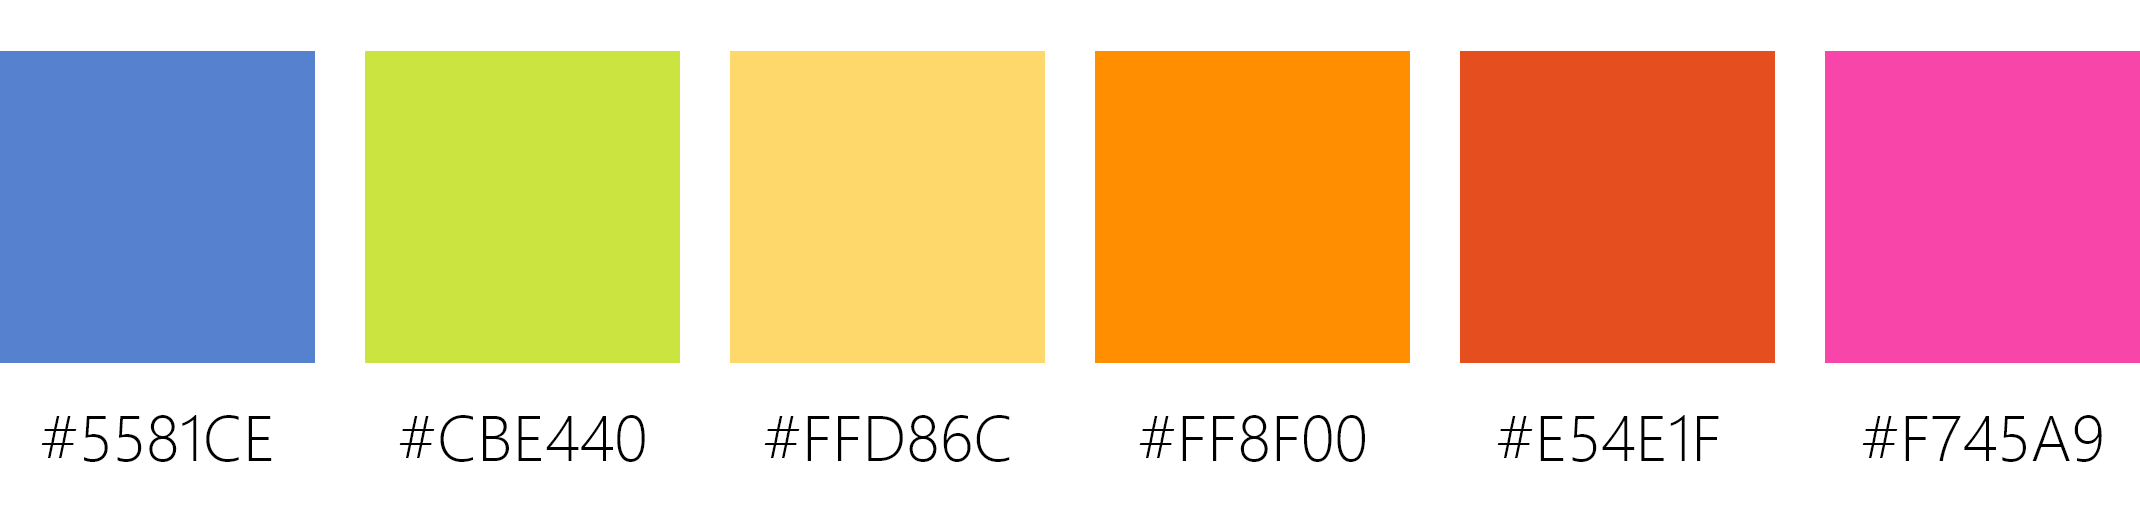
\includegraphics[width=12cm]{Farben.PNG}
\caption{Verwendete Farbpalette}
\label{fig:farben}
\end{figure}

In unserem Fall wurde der Styleguide hauptsächlich zur Dokumentation der Schrift- und Farbvorgaben genutzt. Da sich TraWo in erster Linie an Kinder richtet, war es besonders wichtig, das Farbschema bunt und ansprechend zu halten. Abbildung \ref{fig:farben} zeigt das gewählte Farbschema.

\begin{figure} [h]
\centering
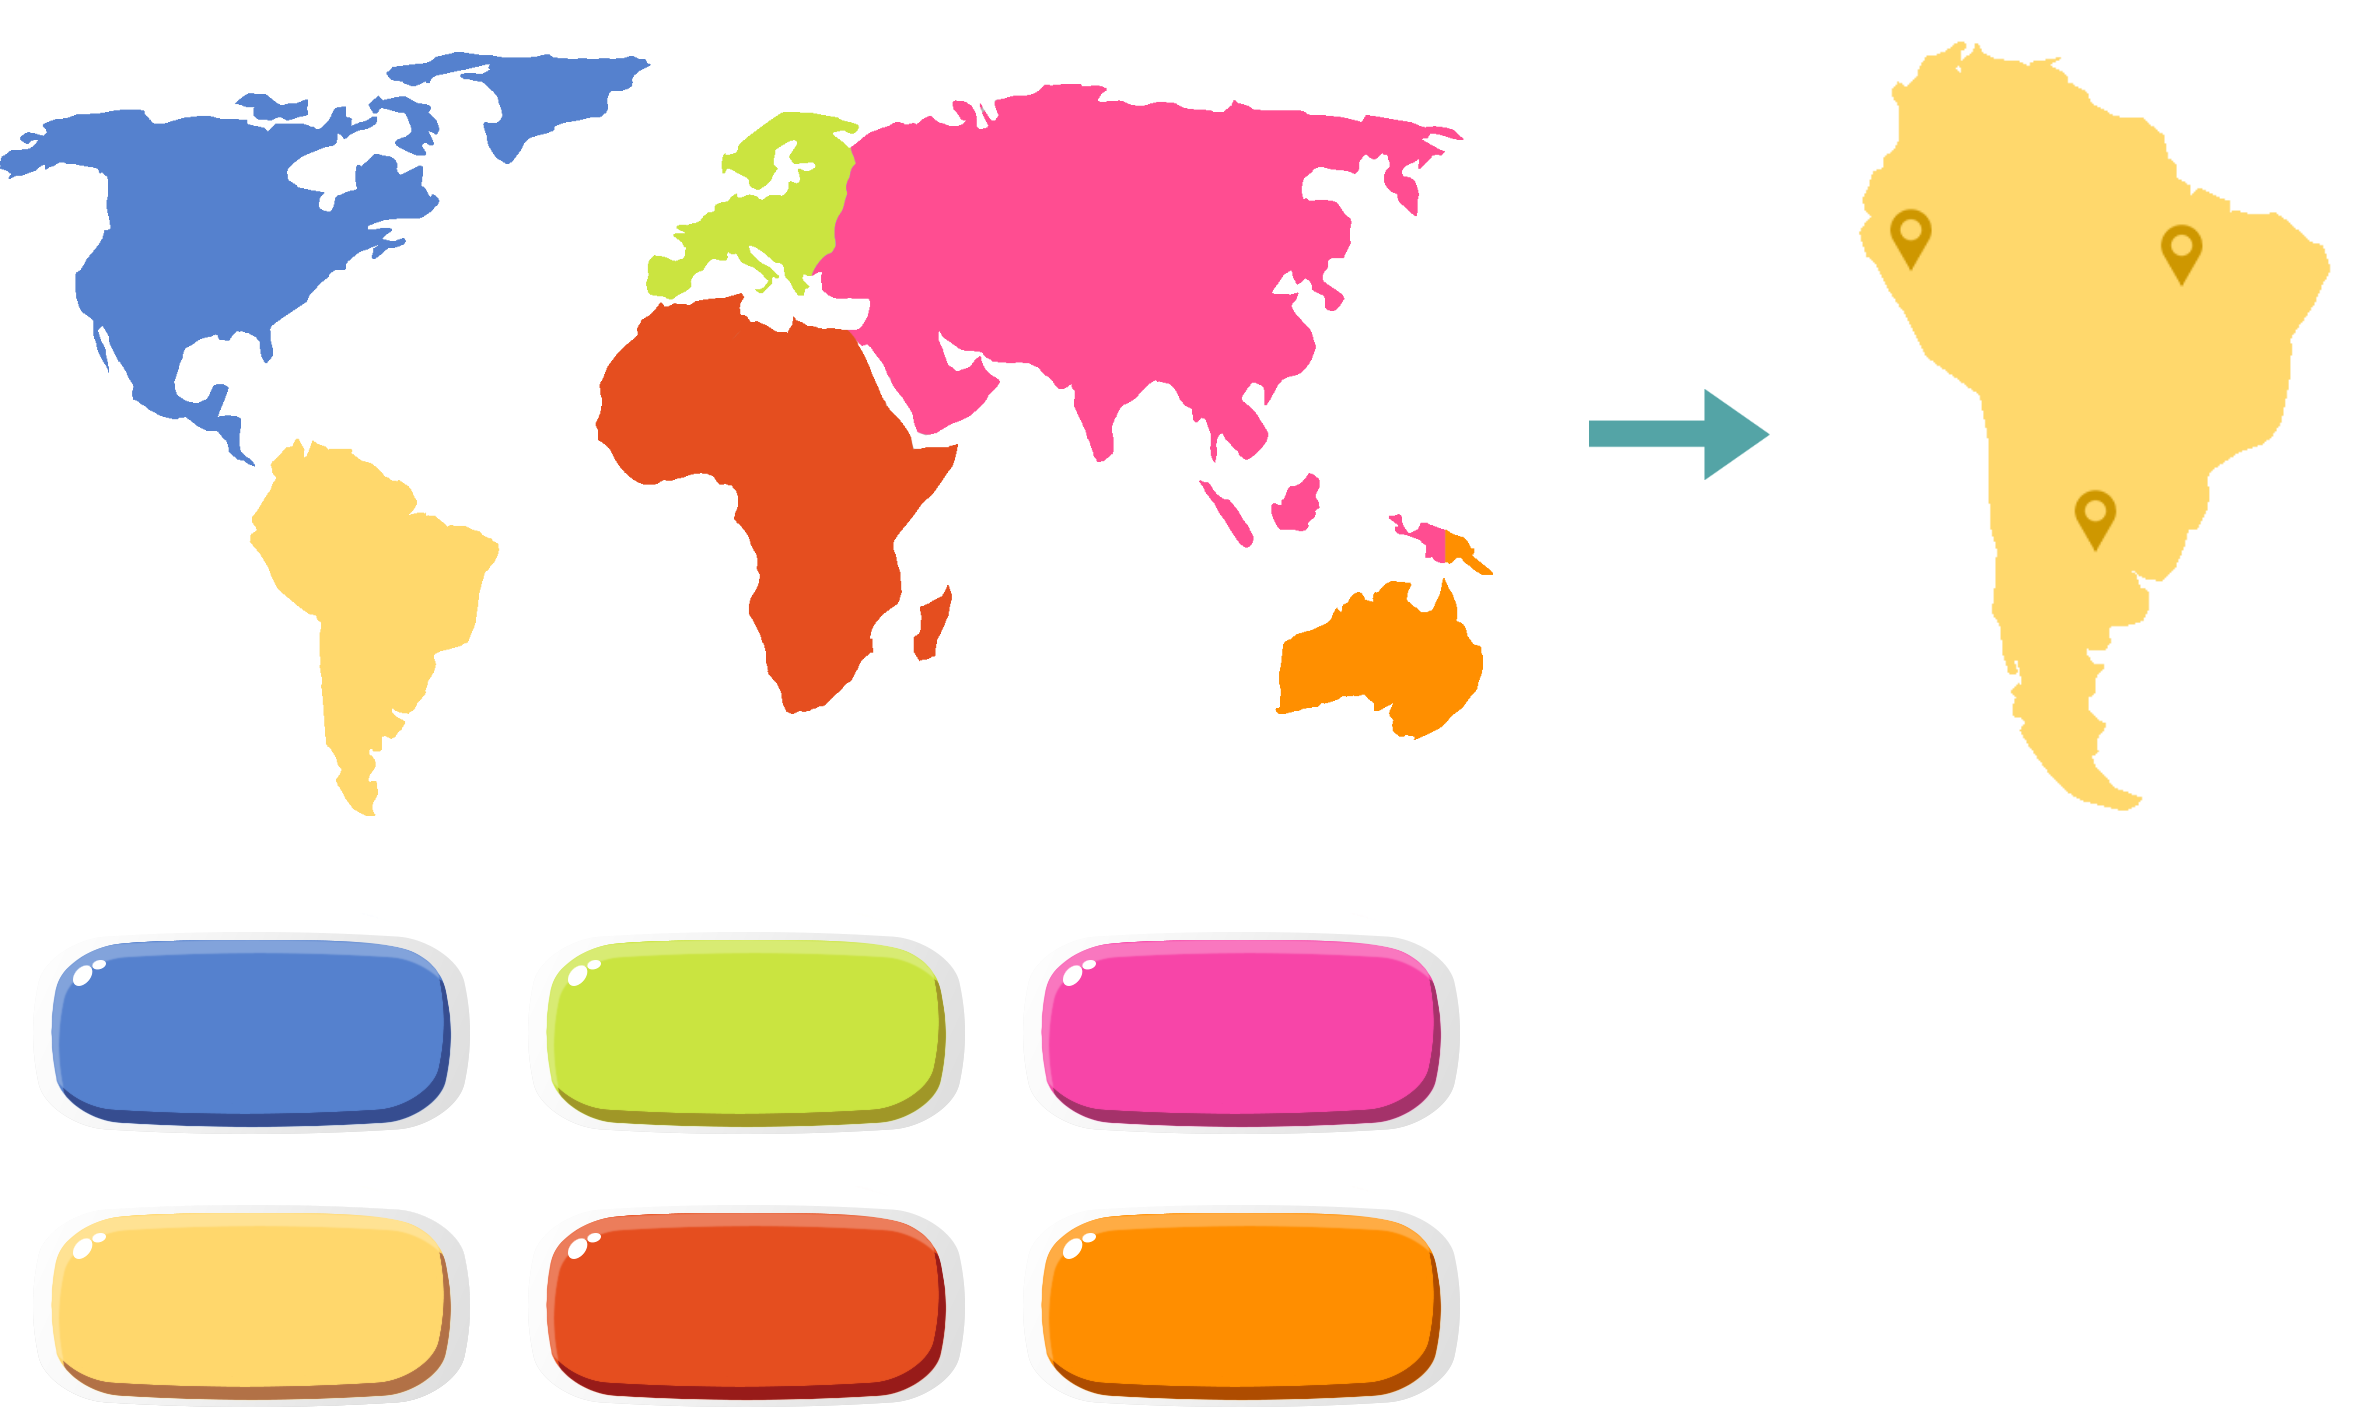
\includegraphics[width=13cm]{Map.PNG}
\caption{Landkarte und Buttons in dem genannten Farbschema}
\label{fig:map}
\end{figure}

Wie in Abbildung \ref{fig:map} zu sehen, ist wurde die oben genannte Farbpalette auf die Landkarte und die Buttons übertragen. Diese sind nur im Informationsteil der Anwendung zu sehen. Die Farben sollen vor allem zum Verständnis der Landkarte dienen und durch die Buttons zeigen, wo sich welcher Kontinent befindet. Nach der Wahl eines Kontinents soll durch Standortsymbole gekennzeichnet werden, welche Länder zur Auswahl stehen.

\subsection{Prototyp}\label{prototyp}
Ein weiterer wichtiger Schritt, der nach einem Styleguide folgt, ist die Entwicklung eines Prototypen. Wie in Abbildung \ref{fig:flowchart} zu sehen, ist wurde dieser in Form eines Flowchart-Models dargestellt.

\begin{figure} [h]
\centering
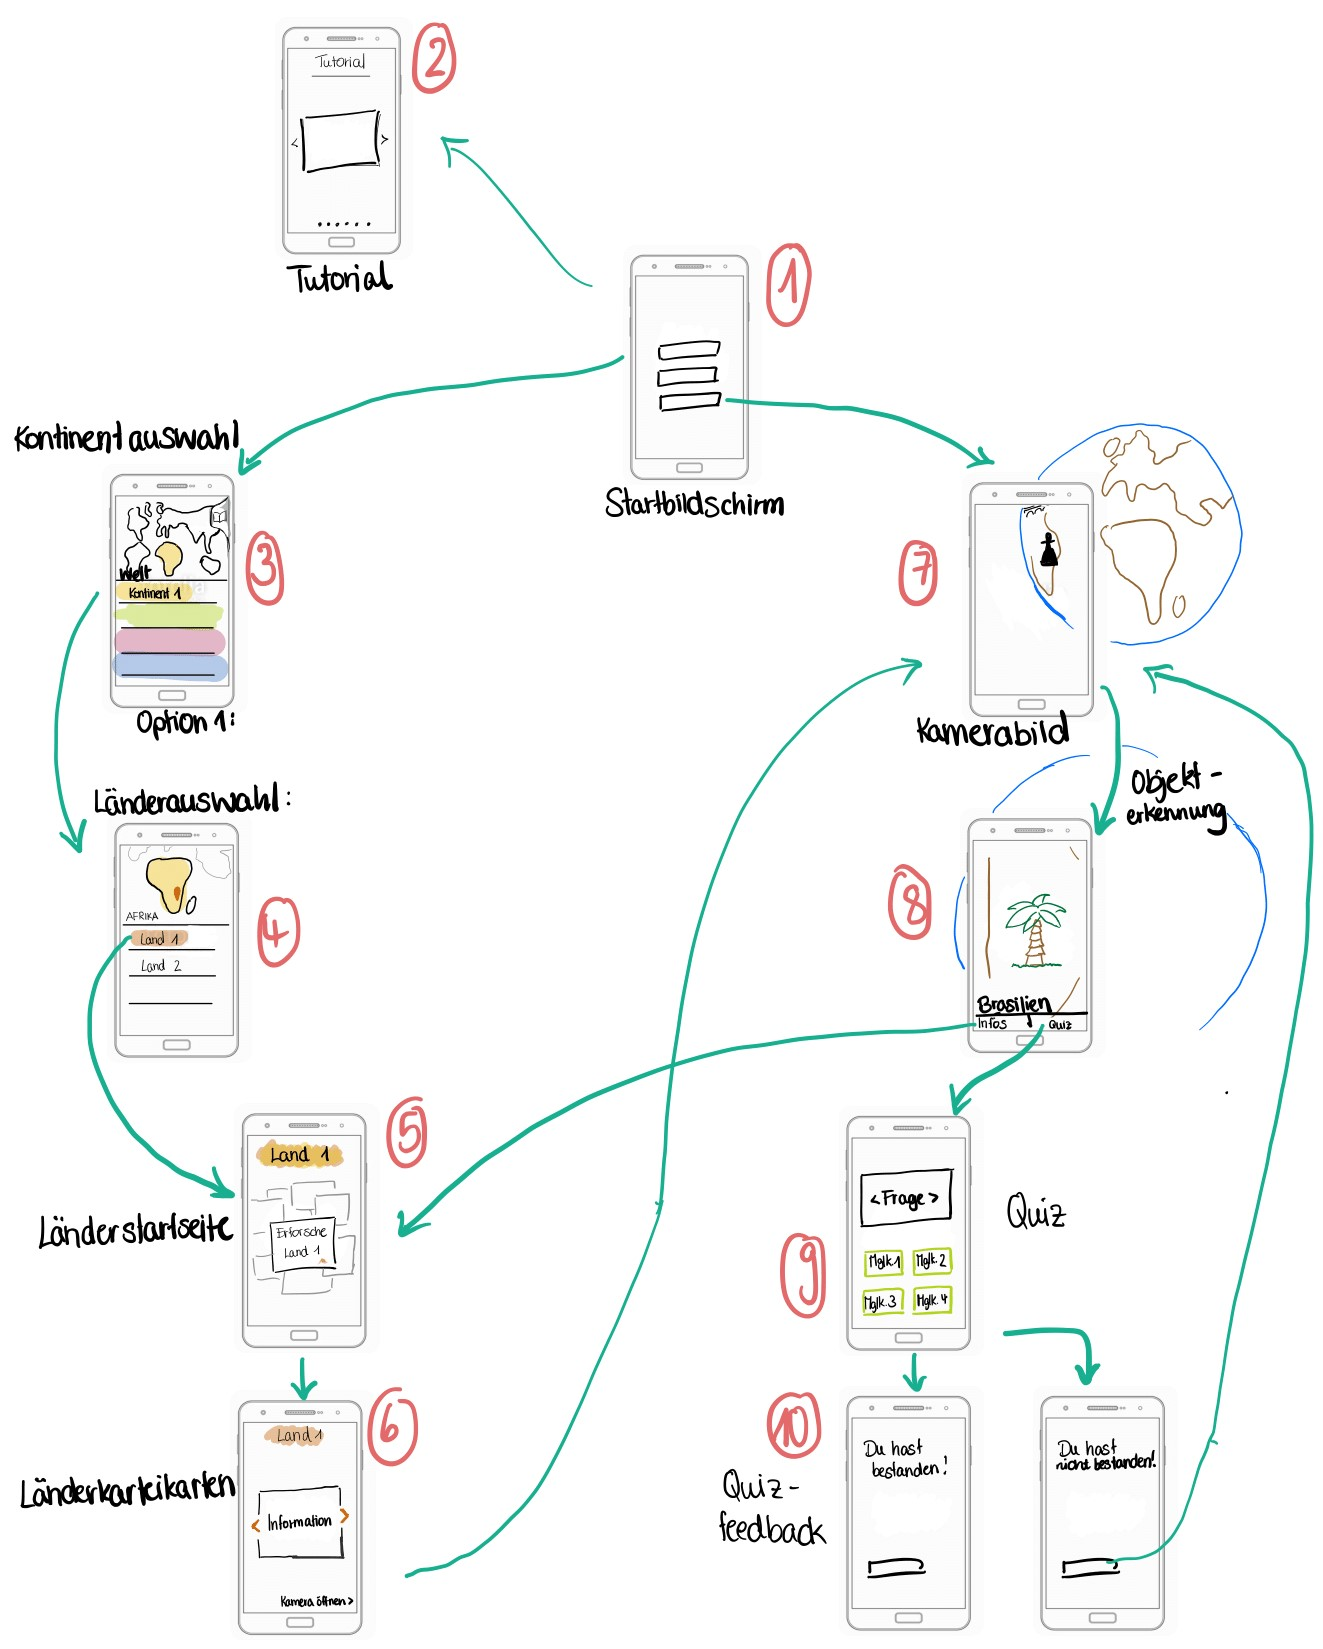
\includegraphics[width=13cm]{flowchart.JPG}
\caption{Prototyp in Form eines Flowchart-Modells}
\label{fig:flowchart}
\end{figure}

Ein Prototyp ist ein Beispiel, das als Grundlage für ein zukünftiges Modell dient. Es bietet die Möglichkeit, die Funktionalität des vorhandenen Designs oder Konzepts vor der Entwicklung zu testen. Somit kann vor allem Zeit gespart werden, falls Änderungswünsche während des Tests auffallen. Außerdem ist es so möglich wertvolle Rückmeldung von anderen Teammitgliedern zu erhalten, bevor das eigentliche Projekt gestartet wird. Ein einfacher Prototyp bietet außerdem mehr Freiraum bei der Entwicklung und vermeidet an kleinen Details hängen zu bleiben. In unserem Fall wurde der Prototyp hauptsächlich dazu genutzt einen groben Überblick für das Team zu schaffen. So hat man bereits eine Vorstellung, wie das fertige Produkt ausschauen könnte und kann im Anschluss ohne Probleme mit der Entwicklung loslegen.

Der Prototyp wurde mithilfe der Anforderungen in den User Stories aus Abschnitt \ref{inhaltliche_anforderungen} erstellt. Zur Darstellung wurde sich wie bereits erwähnt für ein Flowchart-Modell entschieden. Bei einem Flowchart handelt es sich um eine grafische Darstellung des Prozesses, der die Schritte und Funktionen der einzelnen Fenster beschreibt.

Wie man in Abbildung \ref{fig:flowchart} erkennen kann, beginnt die Anwendung mit einem klassischen Hauptmenü. Von dem Menü aus ist es möglich, mit einem Tutorial zu beginnen. Dieses beschreibt in kurzen Sätzen die Funktionalität von TraWo. Ansonsten teilt sich die Anwendung in zwei Teilbereiche auf. Zum einen gelangt man in den Informationsteil, welcher von den Punkten drei bis sechs zu sehen ist. Der Nutzer entscheidet sich zunächst für einen Kontinent und wird anschließend zur Länderauswahl weitergeleitet. Von da aus gelangt er zu den Lernkarten, die die Informationen zu dem gewählten Land wiedergeben. Der zweite Teilbereich, der von den Punkten sieben bis zehn zu sehen ist, beschreibt den Augmented Reality Teil. Von hier aus ist es möglich, zum Quiz zu gelangen. Anschließend führt dieses den Nutzer je nach Ergebnis zum jeweiligen Feedback Fenster.


\section{Architekturentscheidung} \label{architekturentscheidung}
Um die inhaltlichen und grafischen Anforderungen von TraWo realisieren zu können, mussten wir uns auf eine Entwicklungsumgebung, sowie genutzte Frameworks zur Nutzung von Augmented-Reality-Elementen einigen. Der folgende Abschnitt beschreibt das durchgeführte Evaluationsverfahren zur Auswahl einer IDE und benötigten Tools.
\subsection{Entwicklungsumgebung}\label{entwicklungsumgebung}
Für die Entwicklungsumgebung haben sich von Anfang an zwei Favoriten herauskristallisiert. Die Wahl bestand zwischen der Gaming-Engine Unity und der Adroid Studio IDE. Im folgenden werden Vor- und Nachteile der beiden Plattformen aufgelistet.
\subsection{Mustererkennung}
\subsection{Datenhaltung und -bereitstellung}\label{datenhaltung und -bereitstellung}
